\documentclass[aps,prc,reprint,floatfix,nobalancelastpage]{revtex4-1}

\usepackage{siunitx}
\usepackage{amsmath}
\usepackage{mathtools}
\usepackage{algorithm}
\usepackage{algpseudocode}
\usepackage{url}
\frenchspacing

\newcommand{\sun}[0]{\ensuremath{\odot}}

\begin{document}

\title{Project 4: $N$-body simulation of an open galactic cluster}
\author{Joshua Bradt}
\noaffiliation
\date{April 29, 2016}

\begin{abstract}
    A code was developed to model the motion of stars in an open galactic cluster using Newtonian gravity and the Runge-Kutta method of numerical integration. The calculation began with a uniform distribution of stars and found that the system quickly collapsed into a smaller region of space before expanding outward again. The system approached equilibrium toward the end of the calculation, but did not quite reach it. After discussing these results, some possible improvements to the calculation are proposed.
\end{abstract}

\maketitle

\section{Introduction}
\label{sec:introduction}

    An open galactic cluster is a group of similar-mass stars bound together by the gravitational force. These are interesting to astronomers since they provide a well-defined environment for studying the processes of star formation. \cite{Hjorth-Jensen2016} For the purposes of this paper, these clusters also serve as a simple yet physically relevant many-body system that can be easily simulated using basic Newtonian mechanics.

\section{Methods}
\label{sec:methods}

    As described in the report for Project 3, a system of $N$ bodies interacting via the gravitational force can be described in Cartesian coordinates using the $3N$ coupled second-order ordinary differential equations \cite{Project3}
    \begin{align*}
        \frac{d^2 x_k}{dt^2} &= \sum_{i \neq k} \frac{G m_i}{r_{ik}^3} (x_i - x_k) \\
        \frac{d^2 y_k}{dt^2} &= \sum_{i \neq k} \frac{G m_i}{r_{ik}^3} (y_i - y_k) \\
        \frac{d^2 z_k}{dt^2} &= \sum_{i \neq k} \frac{G m_i}{r_{ik}^3} (z_i - z_k)
    \end{align*}
    where
    \begin{equation*}
        r_{ik} = \sqrt{(x_i - x_k)^2 + (y_i - y_k)^2 + (z_i - z_k)^2}.
    \end{equation*}
    Whereas in Project 3 each of these bodies represented a planet orbiting the Sun, in this case, each represents a single star or a small group of stars \cite{Hjorth-Jensen2016}.

    Once the equations above are established, the system can be solved using a variety of different methods. One of the most stable \cite{Project3} and easily implemented \cite{Hjorth-Jensen2016} methods is the fourth-order Runge-Kutta method (RK4), which is described below: (reproduced from \cite{Project3})
    \begin{algorithm}[H]
        \begin{algorithmic}
            \Function{RK4}{$\mathbf{r}$, $\mathbf{v}$, $h$}
                \State $\mathbf{k}_1^v \gets \text{findAcceleration}(\mathbf{r})$
                \State $\mathbf{k}_1^r \gets \mathbf{v}$
                \State $\mathbf{k}_2^v \gets \text{findAcceleration}(\mathbf{r} + \frac{h}{2}\mathbf{k}_1^r)$
                \State $\mathbf{k}_2^r \gets \mathbf{v} + \frac{h}{2} \mathbf{k}_1^v$
                \State $\mathbf{k}_3^v \gets \text{findAcceleration}(\mathbf{r} + \frac{h}{2}\mathbf{k}_2^r)$
                \State $\mathbf{k}_3^r \gets \mathbf{v} + \frac{h}{2} \mathbf{k}_2^v$
                \State $\mathbf{k}_4^v \gets \text{findAcceleration}(\mathbf{r} + h\mathbf{k}_3^r)$
                \State $\mathbf{k}_4^r \gets \mathbf{v} + h \mathbf{k}_3^v$
                \State $\mathbf{v}' \gets \mathbf{v} + \frac{h}{6} (\mathbf{k}_1^v + 2\mathbf{k}_2^v + 2\mathbf{k}_3^v + \mathbf{k}_4^v)$
                \State $\mathbf{r}' \gets \mathbf{r} + \frac{h}{6} (\mathbf{k}_1^r + 2\mathbf{k}_2^r + 2\mathbf{k}_3^r + \mathbf{k}_4^r)$
                \State \textbf{return} $(\mathbf{r}', \mathbf{v}')$
            \EndFunction
        \end{algorithmic}
        \caption{RK4 method for position and velocity}
        \label{alg:rk4}
    \end{algorithm}
    At each time step, this algorithm can be used to update the position and velocity of each particle.

    One problem that can arise in this calculation is numerical instability when two particles move close together, causing $r_{ik} \rightarrow 0$. One way to prevent this is to add a small constant to the gravitational force to prevent the denominator from vanishing. This leads to an expression of the form
    \begin{equation}
        \mathbf{F}_{ik} = \frac{G m_i m_k}{r_{ik}^3 + \epsilon^3} \mathbf{r}_{ik} \label{eq:corrforce}
    \end{equation}
    for the force vector on each particle.

\section{Results}
\label{sec:results}

    I developed a program to simulate this system by repurposing the code from the previous project. \cite{Bradt2016} A system of 500 interacting particles was simulated with a normal initial mass distribution of mean mass $10 m_\sun$ and standard deviation $1 m_\sun$. The initial positions were uniformly distributed inside a sphere of radius \SI{20}{ly}, and the particles started at rest. The simulation progressed with a time step of \SI{0.1}{Ma}.

    Before performing calculations, a value for the parameter $\epsilon$ in (\ref{eq:corrforce}) needed to be found. The value $\epsilon = \SI{0.1}{ly}$ was found by trial and error to be the smallest value that prevented the output from containing discontinuities in particle kinetic energy. This value was used in the remaining calculations discussed in this section.

    \begin{figure}[p]
        \centering
        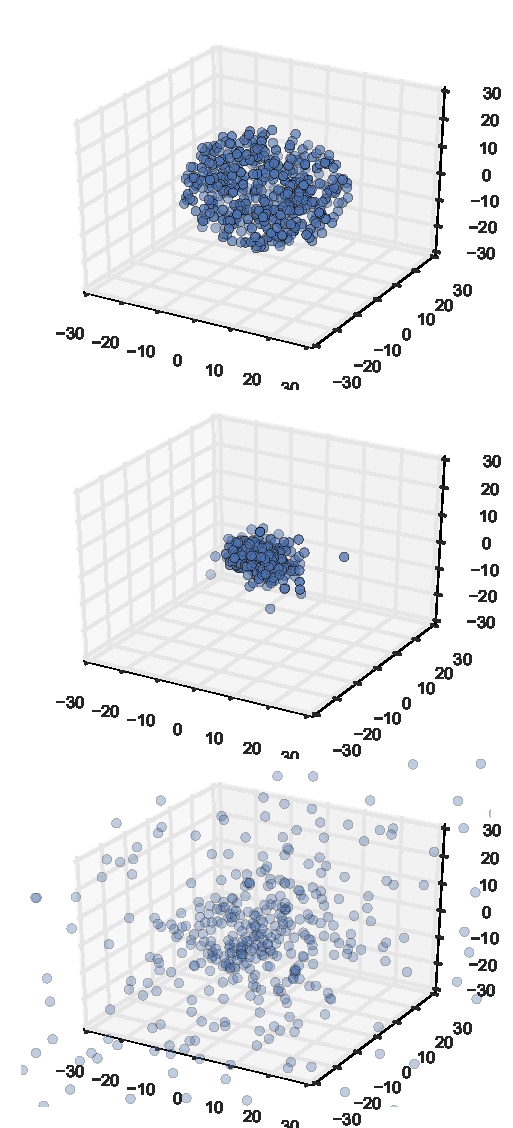
\includegraphics{3d.pdf}
        \caption{Snapshots of the particles' positions at $t=\SI{0}{Ma}$ (top), $t=\SI{5}{Ma}$ (middle), and $t=\SI{199.9}{Ma}$ (bottom). The particles begin uniformly distributed over a sphere, collapse into a smaller volume, and then scatter as some are ejected and others reach an equilibrium.}
        \label{fig:3d}
    \end{figure}

    Three snapshots of the particle distribution are shown in Figure~\ref{fig:3d}. The top image shows the initial conditions, which were uniformly distributed over a sphere. The middle image shows that the particles initially move inward and collapse to a smaller volume. This collapse is also visible in Figure~\ref{fig:rads}, which shows the radial positions of the particles as a function of time. Finally, the particles expand back outwards.

    \begin{figure}[p]
        \centering
        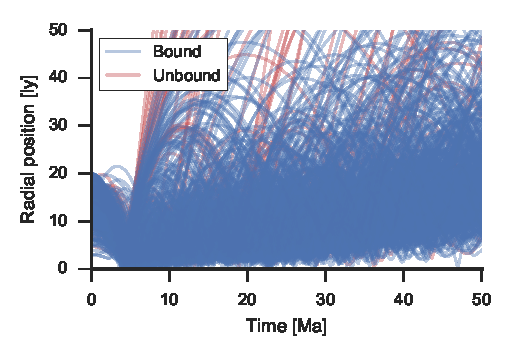
\includegraphics{rads.pdf}
        \caption{Radial positions of the simulated particles.}
        \label{fig:rads}
    \end{figure}

    \begin{figure}[p]
        \centering
        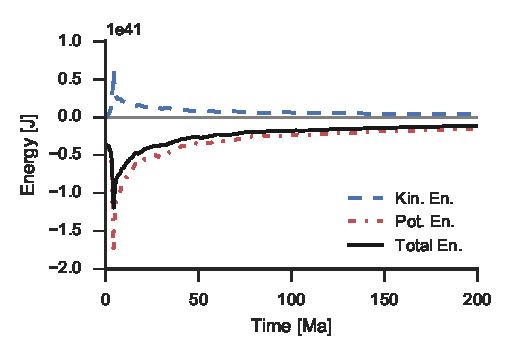
\includegraphics{boundEnergy.pdf}
        \caption{Kinetic, potential, and total energy of the gravitationally bound particles as a function of time.}
        \label{fig:boundEnergy}
    \end{figure}

    The energy of the system is shown in Figure~\ref{fig:boundEnergy} as a function of time. This plot only includes contributions from particles that remained gravitationally bound in the system for the duration of the simulation. Ejected particles identified by looking for particles whose total energy became positive at any point during the simulation. As shown in the figure, the system appears to approach equilibrium after around \SI{50}{Ma}. However, the total energy does appear to be asymptotically approaching zero, which may indicate that particles continue to be ejected even at large times.

    According to the virial theorem, if a system is in equilibrium, then
    \begin{equation}
        2\langle T \rangle + \langle U \rangle = 0, \label{eq:virial}
    \end{equation}
    where the angle brackets indicate a time average, or, by the ergodic hypothesis, an ensemble average. \cite{Hjorth-Jensen2016} Figure~\ref{fig:virial} shows a plot of this function over time for the bound particles. The curve approaches zero at large times, but never quite reaches it. This indicates that the system is approaching equilibrium, but has not quite reached it yet.

    \begin{figure}[p]
        \centering
        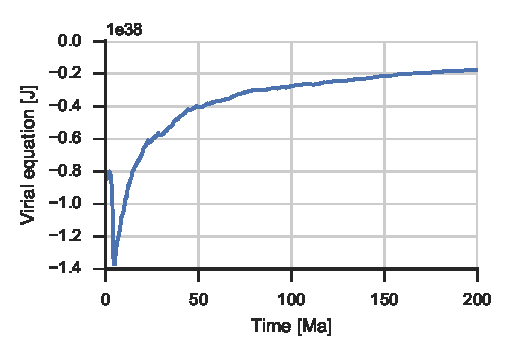
\includegraphics{virial.pdf}
        \caption{Plot of the quantity $2\langle T \rangle + \langle U \rangle$ over time, which should equal zero when the system is in equilibrium if the virial theorem holds.}
        \label{fig:virial}
    \end{figure}

    The number density of the particles is plotted in Figure~\ref{fig:dens} as a function of radial coordinate for the last simulated time step, time $t = \SI{199.9}{Ma}$. The radial coordinate, in this case, is relative to the center of mass of the distribution of bound particles, rather than relative to the initial center of the distribution. This correction was necessary because the center of mass of the system drifted over time as particles were ejected. The distribution was fit using the function
    \begin{equation}
        n(r) = \frac{n_0}{1 + \left(\frac{r}{r_0}\right)^4},
    \end{equation}
    resulting in the parameters $r_0 = \SI{15.09}{ly}$ and $n_0 = \num{8.623e-3}{ly^{-3}}$. The fit is quite good outside of approximately $r = \SI{10}{ly}$, but the distribution does not follow the fit function closer to the center of mass.

    \begin{figure}[p]
        \centering
        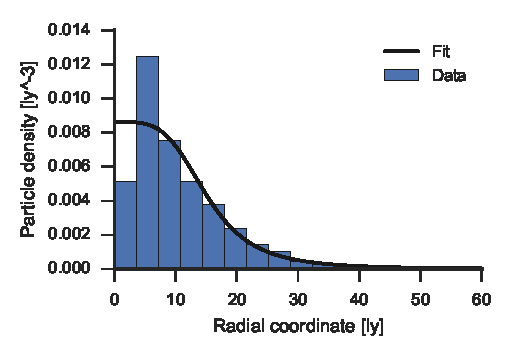
\includegraphics{dens.pdf}
        \caption{Number density of particles as a function of the radial distance from the system's center of mass at time $t=\SI{199.9}{Ma}$. The fit shown is the function $n(r) = \frac{n_0}{1 + (r / r_0)^4}$ where $r_0 = \SI{15.09}{ly}$ and $n_0 = \num{8.623e-3}{ly^{-3}}$.}
        \label{fig:dens}
    \end{figure}

\section{Conclusion}
\label{sec:conclusion}

    A code was written to simulate the motion of stars under the influence of gravity in an open galactic cluster. The forces on the stars were calculated using a simple Newtonian model of gravity. The results show the simulated particles initially collapsing into a smaller region of space before expanding outward again and achieving something close to equilibrium.

    There are many clear improvements that could be made to this code. Most importantly, the model used completely neglects relativistic effects, which is likely a poor approximation to reality when dealing with such massive objects. A more sophisticated model might also take the extent of the stars into account instead of treating them as point-like particles. Additionally, the algorithm could possibly be made more efficient, at least with respect to memory access, by representing the cluster of particles as a contiguous data structure like a matrix rather than a disparate set of objects scattered around in memory. The computations could also likely be parallelized without too much effort, thereby speeding up the code and increasing the number of particles that can be handled.

\bibliography{project4.bib}


\end{document}
